\documentclass[12pt]{article}
\usepackage{verbatim}
\usepackage[dvips]{epsfig}
\usepackage{color}
\usepackage{url}
\usepackage[colorlinks=true]{hyperref}

\begin{document}

\section*{GENESIS: Documentation}

{\bf Related Documentation:}
% start: userdocs-tag-replace-items related-do-nothing
% end: userdocs-tag-replace-items related-do-nothing

\section*{De Schutter: Purkinje Cell Model}

\begin{figure}[h]
\centering
   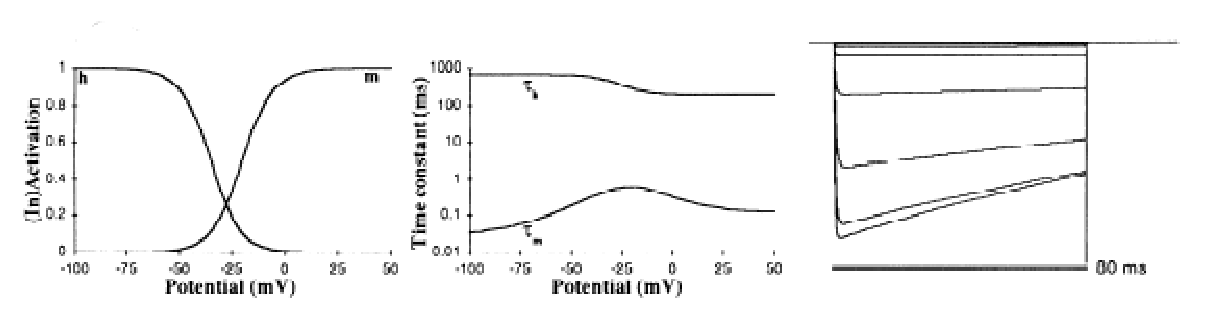
\includegraphics[scale=0.75]{figures/DS1.2C.eps}
   \caption{Activation and inactivation properties of the P-type calcium (CaP, ---) ionic conductances in the model. Seady-state activation and inactivation vs. voltage are plotted at the {\em left}, the time constants of activation ($\tau_m$) and inactivation ($\tau_h$) vs. voltage in the {\em middle} (Note: Semilogarithmic scale), and a simulation of representative voltage-clamp currents at the {\em right}, obtained from a spherical cell and assuming a complete block of all other channels. They simulate steps from a holding potential of -110 to -70\,mV up to 0\,mV in 10\,mV increments. The voltage-clamp current amplitude has been scaled arbitrarily because we mainly wanted to demonstrate the current kinetics.}
   \label{fig:DS1.2C}
\end{figure}

\subsection*{P-Type Calcium Current}

The P-type Ca$^{2+}$ channel is a high-threshold, very slowly inactivating channel first described in the Purkinje cell\,\cite{R:1980ly}. A complete whole-cell patch clamp study of this channel in freshly dissociated rat Purkinje cells was done by\,\cite{Regan:1991ly}; this provided us with all the data necessary to model the P-type calcium (CaP) current (Fig. 2$C$). Initial versions of the model were run with equations based on averaged data\,\cite{Regan:1991ly} but, confirming our experience in other systems\,\cite{De-Schutter-E:1993fu}, we found that equations based on data from a single preparation (Figs. 5$C$ and 6$C$ in\,\cite{Regan:1991ly}) made Ca$^{2+}$ spiking in the model more robust. These data do not support multiple activation states for the CaP channel because there does not seem to be any delay in activation\,\cite{hodgkin52:_quantitative_description} and the steady-state activation curve could be fitted by a Boltzmann-style curve with power 1. Therefore activation of CaP has been modeled with a single gate. This is in contrast to equations for other mammalian Ca$^{2+}$ currents, which usually show some delay in activation\,\cite{Chen:1990ve, Kay:1987ar}.

Recently,\,\cite{Usowicz:1992bh, Usowicz:1992qf} also reported CaP channel data on the basis of cell-attached patch clamps of guinea pig Purkinje cells. These results seem to be in accord with the data reported by\,\cite{Regan:1991ly} for activation; the threshold of activation especially is very similar (-41\,mV in 2\,mM Ca$^{2+}$ reported by Usowicz et al.\,\cite{Usowicz:1992bh} vs. -45 to -40\,mV in 5\,mM Ba$^{2+}$\,\cite{Regan:1991ly}. However, Usowicz et al.\,\cite{Usowicz:1992qf} show little or no inactivation of CaP current, whereas\,\cite{Regan:1991ly} declares that there is a slow inactivation. Other authors claim that there might be several time constants of inactivation for CaP current\,\cite{Hockberger:1991dq} and to our knowledge a possible Ca$^{2+}$-dependent inactivation, as found in other high-threshold Ca$^{2+}$ channels\,\cite{Fox:1987zr} has not been completely excluded. The model used the slow inactivation suggested by\,\cite{Regan:1991ly} (Fig. 2$C$).

\bibliographystyle{plain}
\bibliography{../tex/bib/g3-refs}

\end{document}
